


\begin{minipage}{\linewidth}
\center{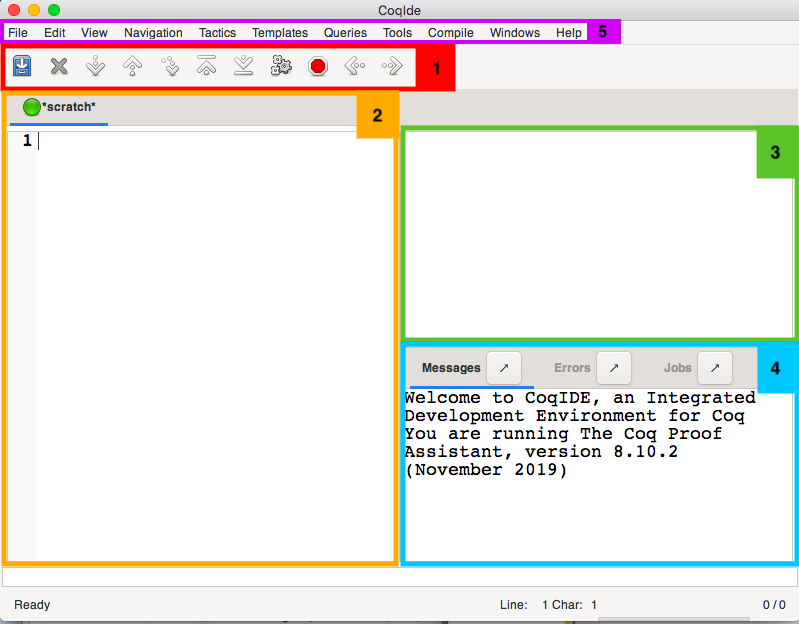
\includegraphics[width=\textwidth]
        {CoqScreenshots/CoqIDEv8_10_2_color.png}}
        \label{fig:IDEcolor} 
        \captionof{figure}{\TT{CoqIDE v8.10.2}:  
        (1) Toolbar. (2) Script Buffer. (3) Goal Window. (4) Message Window. \\ (5) Menu Bar.}
\end{minipage}




\subsection{Toolbar for CoqIDE v8.10.2} \label{subsec: toolbar}
\hspace{-0.75cm}
\begin{tabular}{ C L }
\centered{
\includegraphics[width=\iconsize]
        {CoqScreenshots/save_10.png}}
        & \centeredl{\TT{Save current buffer.} 
        If it hasn't been previously saved, functions as save as; use the extension .v to save as a Coq file.
        } \\ \\
\centered{
\includegraphics[width=\iconsize]
        {CoqScreenshots/close_10.png}}
	& \centeredl{\TT{Close current buffer.} 
	Gives a warning if the file has unsaved changes.
	} \\ \\
\centered{
\includegraphics[width=\iconsize]
        {CoqScreenshots/step_forward_10.png}}
	& \centeredl{\TT{Forward one command.}
	Steps forward to evaluate the next command in the current file.
	} \\ \\
\centered{
\includegraphics[width=\iconsize]
        {CoqScreenshots/step_backward_10.png}}
	& \centeredl{\TT{Backward one command.}
	Steps backward one command in the file, returns the state to where it was before evaluating that command. 
	} \\ \\ 
\centered{
\includegraphics[width=\iconsize]
        {CoqScreenshots/go_to_cursor_10.png}}
	& \centeredl{\TT{Go to cursor.}
	Evaluate all commands in file up to where the cursor currently is.
	} \\ \\ 
\centered{
\includegraphics[width=\iconsize]
        {CoqScreenshots/go_to_top_10.png}}
	& \centeredl{\TT{Restart Coq.}
	Returns to the top of the file, where no commands have been evaluated.
	} \\ \\ 
\centered{
\includegraphics[width=\iconsize]
        {CoqScreenshots/go_to_bottom_10.png}}
	& \centeredl{\TT{Go to end.}
	Evaluate to the bottom of the file. 
	Does not work as well with load commands and require import commands.
	} \\ \\
\centered{
\includegraphics[width=\iconsize]
        {CoqScreenshots/check_10.png}}
	& \centeredl{\TT{Fully check the document.}
	Submits proof terms to the Coq kernel for type checking.
	} \\ \\
\centered{
\includegraphics[width=\iconsize]
        {CoqScreenshots/stop_10.png}}
	& \centeredl{\TT{Interrupt computations.}
	Stops computation at whatever point was reached before pressing the button.
	} \\ \\
\centered{
\includegraphics[width=\iconsize]
        {CoqScreenshots/next_occurrence_10.png}}
	& \centeredl{\TT{Next Occurrence.}
	Goes to the next occurrence of whatever the cursor is currently by. 
	Works well for longer words.
	} \\ \\
\centered{
\includegraphics[width=\iconsize]
        {CoqScreenshots/previous_occurrence_10.png}}
	& \centeredl{\TT{Previous Occurrence.}
	Goes to the previous occurrence of whatever the cursor is currently by.
	Works well for longer words.
	}
\end{tabular}





















